\documentclass[tikz,border=5pt]{standalone}
\usepackage[UTF8]{ctex}
\usepackage{amsmath,amssymb}
\usetikzlibrary{arrows.meta,calc,angles,quotes,decorations.pathmorphing,patterns}
\definecolor{ink}{HTML}{243447}\definecolor{blue}{HTML}{2765A2}
\definecolor{green}{HTML}{3F7D5B}\definecolor{red}{HTML}{B74739}
\tikzset{body/.style={draw=ink,thick},vec/.style={draw=blue,thick,-{Latex}},guide/.style={gray!65,dashed},dim/.style={ink,{Latex}-{Latex}},line cap=round,line join=round}
\begin{document}

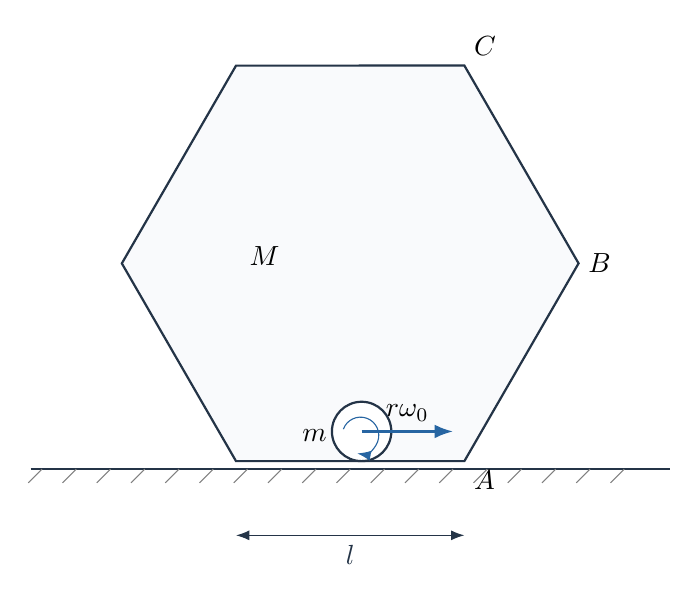
\begin{tikzpicture}[scale=1.45]
\coordinate(A)at(1,0);\coordinate(B)at(2,1.732);\coordinate(C)at(1,3.464);
\draw[body,fill=blue!3](-1,0)--(A)--(B)--(C)--(-1,3.464)--(-2,1.732)--cycle;
\draw[body](-2.8,-.07)--(2.8,-.07);
\foreach \x in {-2.7,-2.4,...,2.7}\draw[gray](\x,-.07)--++(-.12,-.12);
\draw[body,fill=white](.1,.26)circle(.26);
\draw[vec](.1,.26)--(.9,.26)node[midway,above]{$r\omega_0$};
\draw[blue,-{Latex}](-.06,.28)arc(160:-100:.16);
\node[left]at(-.12,.22){$m$};\node at(-.75,1.8){$M$};
\node[below right]at(A){$A$};\node[right]at(B){$B$};\node[above right]at(C){$C$};
\draw[dim](-1,-.65)--(1,-.65)node[midway,below]{$l$};
\end{tikzpicture}
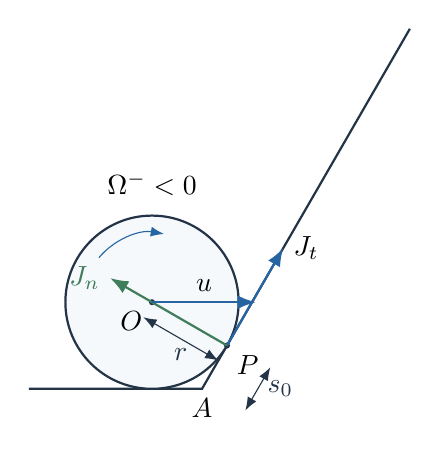
\begin{tikzpicture}[scale=1.1]
\coordinate(A)at(0,0);\coordinate(P)at(.288675,.5);
\coordinate(O)at(-.57735,1);
\draw[body](-2,0)--(A)--(2.4,4.157);
\draw[body,fill=blue!4](O)circle(1);
\fill[ink](P)circle(.035);\fill[ink](O)circle(.035);
\draw[dim]($(O)+(-.1,-.1732)$)--($(P)+(-.1,-.1732)$)node[midway,below]{$r$};
\draw[vec](P)--++(.65,1.126)node[right]{$J_t$};
\draw[green,thick,-{Latex}](P)--++(-1.35,.7794)node[left]{$J_n$};
\draw[vec](O)--++(1.2,0)node[midway,above]{$u$};
\draw[blue,-{Latex}]($(O)+({.8*cos(140)},{.8*sin(140)})$)arc(140:80:.8);
\node[above]at($(O)+(0,1.12)$){$\Omega^-<0$};
\node[below]at(A){$A$};\node[below right]at(P){$P$};\node[below left]at(O){$O$};
\draw[dim](.5,-.25)--(.788675,.25)node[midway,right]{$s_0$};
\end{tikzpicture}
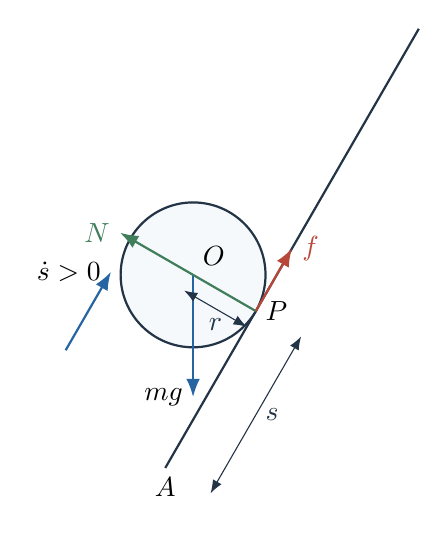
\begin{tikzpicture}[scale=1.15]
\coordinate(A)at(0,0);\coordinate(P)at(1,1.732);\coordinate(O)at(.307,2.132);
\draw[body](A)--(2.8,4.85);
\draw[body,fill=blue!4](O)circle(.8);
\draw[vec](O)--++(0,-1.35)node[left]{$mg$};
\draw[green,thick,-{Latex}](P)--++(-1.5,.866025)node[left]{$N$};
\draw[red,thick,-{Latex}](P)--++(.4,.693)node[right]{$f$};
\draw[dim]($(O)+(-.1,-.1732)$)--($(P)+(-.1,-.1732)$)node[midway,below]{$r$};
\draw[vec](-1.1,1.3)--++(.5,.866)node[left]{$\dot s>0$};
\node[above right]at(O){$O$};\node[right]at(P){$P$};\node[below]at(A){$A$};
\draw[dim](.5,-.28)--(1.5,1.452)node[midway,right]{$s$};
\end{tikzpicture}
\begin{tikzpicture}[scale=1.2]
\draw[body,fill=blue!3](-1,0)--(1,0)--(2,1.732)--(1,3.464)--(-1,3.464)--(-2,1.732)--cycle;
\coordinate(P)at(1.8,1.386); \fill[ink](P)circle(.04);
\draw[red,thick,-{Latex}](P)--++(.52,-.9)node[right]{$\boldsymbol F_{\text{筒}}$};
\draw[vec](0,1.732)--(0,.5)node[left]{$Mg$};
\draw[guide](P)--(1.8,-.25);\draw[guide](P)--(0,1.386);
\draw[vec](.7,0)--(.7,.95)node[left]{$N_g$};
\draw[green,thick,-{Latex}](.7,0)--(-.2,0)node[below]{$F_g$};
\draw[body](-2.6,-.06)--(2.6,-.06);
\draw[dim](0,-.65)--(.7,-.65)node[midway,below]{$\xi$};
\draw[dim](-1,-1.3)--(1,-1.3)node[midway,below]{$l$};
\node[below right]at(1,0){$A$};\node[above right]at(P){$P$};
\node[left]at(0,1.386){$y_P$};\node[below right]at(1.8,-.23){$x_P$};
\end{tikzpicture}
\end{document}
